\section{Implementation of Defeaturing System} \label{sec:defeaturing:implementation}
Prototype implementation has been done using Application Programming Interface (APIs) of Autodesk Inventor \textsuperscript{\textregistered}, in Microsoft Visual Basic .Net 2010 environment on 2.3 GHz Intel i3, 64 bit processor PC with 4 GB RAM.  Many of the example parts have been borrowed from GrabCAD\textsuperscript{\textregistered} site (http://www.grabcad.com).

\vspace{3mm}

\begin{minipage}[t]{\linewidth}
\begin{tabular}[tb]{@{} p{0.7\linewidth} p{0.25\linewidth}@{}}

\adjustbox{valign=t}{
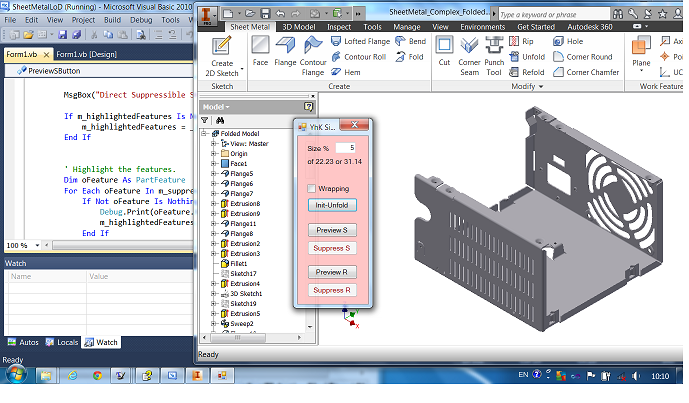
\includegraphics[width=\linewidth]{../Common/images/ImplDefeaturingProgram.png}}

&
\adjustbox{valign=t}{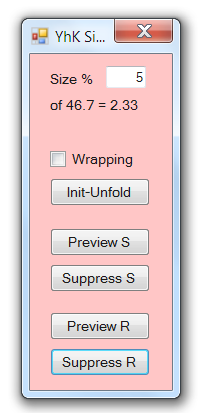
\includegraphics[width=0.8\linewidth]{../Common/images/DefeaturingDialog.png}}\\
\end{tabular}
 \captionof{figure}{Screen-shot of implemented program} \label{fig:defeaturing:implementation}
\end{minipage}

\bigskip

The implemented (Fig. ~\ref{fig:defeaturing:implementation}) user work-flow is as follows:
\begin{itemize}
[noitemsep,topsep=2pt,parsep=2pt,partopsep=2pt,label=\textbullet]
\item Input part is loaded.
\item \textbf{Init-Unfold}: Part is Unfold-ed. Its size and thresholds are calculated.
\item \textbf{Preview S}: Phase I-selected (\underline{\bf S}heet metal) features are highlighted
\item \textbf{Suppress S}: The selected (\underline{\bf S}heet metal) features are suppressed.
\item \textbf{Preview R}: Phase II-selected (\underline{\bf R}emnant) features are highlighted
\item \textbf{Suppress S}: The selected (\underline{\bf R}emnant) features are suppressed.
%\item Validation statistics is displayed
\end{itemize}